%8 pages
%%
%% This is file `sample-sigconf.tex',
%% generated with the docstrip utility.
%%
%% The original source files were:
%%
%% samples.dtx  (with options: `sigconf')
%% 
%% IMPORTANT NOTICE:
%% 
%% For the copyright see the source file.
%% 
%% Any modified versions of this file must be renamed
%% with new filenames distinct from sample-sigconf.tex.
%% 
%% For distribution of the original source see the terms
%% for copying and modification in the file samples.dtx.
%% 
%% This generated file may be distributed as long as the
%% original source files, as listed above, are part of the
%% same distribution. (The sources need not necessarily be
%% in the same archive or directory.)
%%
%% The first command in your LaTeX source must be the \documentclass command.
\documentclass[sigconf,table]{acmart}

\usepackage{algpseudocode}
\usepackage{algorithm}
\usepackage{algorithmicx}
\usepackage{verbatim}
\usepackage{mathtools}
\usepackage{multirow}
\usepackage{subcaption}
\usepackage{colortbl}

\usepackage{tikz}
\usetikzlibrary{automata,positioning}

\definecolor{lightgray}{gray}{0.9}


%\def\BibTeX{{\rm B\kern-.05em{\sc i\kern-.025em b}\kern-.08em
	%	T\kern-.1667em\lower.7ex\hbox{E}\kern-.125emX}}

\usepackage{booktabs} % For formal tables


\newlength\Origarrayrulewidth

% horizontal rule equivalent to \cline but with 2pt width
\newcommand{\Cline}[1]{%
	\noalign{\global\setlength\Origarrayrulewidth{\arrayrulewidth}}%
	\noalign{\global\setlength\arrayrulewidth{3pt}}\cline{#1}%
	\noalign{\global\setlength\arrayrulewidth{\Origarrayrulewidth}}%
}

% draw a vertical rule of width 2pt on both sides of a cell
\newcommand\Thickvrule[1]{%
	\multicolumn{1}{!{\vrule width 2pt}c!{\vrule width 2pt}}{#1}%
}

% draw a vertical rule of width 2pt on the left side of a cell
\newcommand\Thickvrulel[1]{%
	\multicolumn{1}{!{\vrule width 2pt}c}{#1}%
}

% draw a vertical rule of width 2pt on the right side of a cell
\newcommand\Thickvruler[1]{%
	\multicolumn{1}{c!{\vrule width 2pt}}{#1}%
}

%%
%% \BibTeX command to typeset BibTeX logo in the docs
\AtBeginDocument{%
	\providecommand\BibTeX{{%
			\normalfont B\kern-0.5em{\scshape i\kern-0.25em b}\kern-0.8em\TeX}}}

%% Rights management information.  This information is sent to you
%% when you complete the rights form.  These commands have SAMPLE
%% values in them; it is your responsibility as an author to replace
%% the commands and values with those provided to you when you
%% complete the rights form.
\setcopyright{acmcopyright}
\copyrightyear{2020}
\acmYear{2020}
\acmConference[GRADES-NDA'20]{Joint Workshop on Graph Data Management Experiences \& Systems (GRADES) and Network Data Analytics (NDA)}{June 14, 2020}{Portland, OR, USA}
\acmBooktitle{Joint Workshop on Graph Data Management Experiences \& Systems (GRADES) and Network Data Analytics (NDA), June 14, 2020, Portland, OR, USA}
\acmPrice{15.00}
\acmDOI{}
\acmISBN{XXX-X-XXXXX-XXX-X}


%%
%% Submission ID.
%% Use this when submitting an article to a sponsored event. You'll
%% receive a unique submission ID from the organizers
%% of the event, and this ID should be used as the parameter to this command.
%%\acmSubmissionID{123-A56-BU3}

%%
%% The majority of ACM publications use numbered citations and
%% references.  The command \citestyle{authoryear} switches to the
%% "author year" style.
%%
%% If you are preparing content for an event
%% sponsored by ACM SIGGRAPH, you must use the "author year" style of
%% citations and references.
%% Uncommenting
%% the next command will enable that style.
%%\citestyle{acmauthoryear}

\newtheorem{mytheorem}{Theorem}

\newcommand{\ltz}{$< 1$}

\algtext*{EndWhile}% Remove "end while" text
\algtext*{EndIf}% Remove "end if" text
\algtext*{EndFor}% Remove "end for" text
\algtext*{EndFunction}% Remove "end function" text

%%
%% end of the preamble, start of the body of the document source.
\begin{document}
	
	%%
	%% The "title" command has an optional parameter,
	%% allowing the author to define a "short title" to be used in page headers.
	\title[]{Context-Free Path Querying with Single-Path Semantics by Matrix Multiplication}
	
	%%
	%% The "author" command and its associated commands are used to define
	%% the authors and their affiliations.
	%% Of note is the shared affiliation of the first two authors, and the
	%% "authornote" and "authornotemark" commands
	%% used to denote shared contribution to the research.
	\author{Arseniy Terekhov}
	\email{simpletondl@yandex.ru}
	\affiliation{%
		\institution{Saint Petersburg State University}
		\streetaddress{7/9 Universitetskaya nab.}
		\city{St. Petersburg}
		\country{Russia}
		\postcode{199034}
	}
	
	
	\author{Artyom Khoroshev}
	\email{arthoroshev@gmail.com}
	\affiliation{%
		\institution{ITMO University}
		\streetaddress{49 Kronverksky prospekt}
		\city{St. Petersburg}
		\country{Russia}
		\postcode{197101}
	}
	
	
	\author{Rustam Azimov}
	\email{rustam.azimov19021995@gmail.com}
	%\email{semyon.grigorev@jetbrains.com}
	%orcid{0000-0002-7966-0698}
	\affiliation{
		\institution{Saint Petersburg State University}
		\streetaddress{7/9 Universitetskaya nab.}
		\city{St. Petersburg}
		\country{Russia}
		\postcode{199034}
	}
	\affiliation{
		\institution{JetBrains Research}
		\streetaddress{Primorskiy prospekt 68-70, Building 1}
		\city{St. Petersburg}
		\country{Russia}
		\postcode{199034}
	}
	
	
	\author{Semyon Grigorev}
	\email{s.v.grigoriev@spbu.ru}
	\email{semyon.grigorev@jetbrains.com}
	\orcid{0000-0002-7966-0698}
	\affiliation{
		\institution{Saint Petersburg State University}
		\streetaddress{7/9 Universitetskaya nab.}
		\city{St. Petersburg}
		\country{Russia}
		\postcode{199034}
	}
	\affiliation{
		\institution{JetBrains Research}
		\streetaddress{Primorskiy prospekt 68-70, Building 1}
		\city{St. Petersburg}
		\country{Russia}
		\postcode{199034}
	}
	
	%%
	%% By default, the full list of authors will be used in the page
	%% headers. Often, this list is too long, and will overlap
	%% other information printed in the page headers. This command allows
	%% the author to define a more concise list
	%% of authors' names for this purpose.
	\renewcommand{\shortauthors}{Terekhov, Khoroshev, Azimov, Grigorev}
	
	%
	% The abstract is a short summary of the work to be presented in the article.
	\begin{abstract}
		A recent study showed that the applicability of context-free path querying (CFPQ) algorithms with relational query semantics integrated with Neo4j database is limited because of low performance and high memory consumption. In this work we implement a matrix-based CFPQ algorithm by using appropriate high-performance libraries for linear algebra and integrate it with RedisGraph graph database. Also, we introduce a new CFPQ algorithm with single-path query semantics that allows us to extract one found path for each pair of nodes. Finally, we provide the evaluation of our algorithms for both semantics which shows that matrix-based CFPQ implementation for RedisGraph database is performant enough for real-world data analysis.
	\end{abstract}
	
	%
	% The code below is generated by the tool at http://dl.acm.org/ccs.cfm.
	% Please copy and paste the code instead of the example below.
	%
	\begin{CCSXML}
		<ccs2012>
		<concept>
		<concept_id>10002951.10002952.10003197.10010825</concept_id>
		<concept_desc>Information systems~Query languages for non-relational engines</concept_desc>
		<concept_significance>500</concept_significance>
		</concept>
		<concept>
		<concept_id>10003752.10003766.10003771</concept_id>
		<concept_desc>Theory of computation~Grammars and context-free languages</concept_desc>
		<concept_significance>500</concept_significance>
		</concept>
		<concept>
		<concept_id>10010147.10010169.10010170.10010174</concept_id>
		<concept_desc>Computing methodologies~Massively parallel algorithms</concept_desc>
		<concept_significance>500</concept_significance>
		</concept>
		<concept>
		<concept_id>10003752.10003753.10003761.10003762</concept_id>
		<concept_desc>Theory of computation~Parallel computing models</concept_desc>
		<concept_significance>300</concept_significance>
		</concept>
		<concept>
		<concept_id>10010520.10010521.10010528.10010534</concept_id>
		<concept_desc>Computer systems organization~Single instruction, multiple data</concept_desc>
		<concept_significance>300</concept_significance>
		</concept>
		</ccs2012>
	\end{CCSXML}
	
	\ccsdesc[500]{Information systems~Query languages for non-relational engines}
	\ccsdesc[500]{Theory of computation~Grammars and context-free languages}
	\ccsdesc[500]{Computing methodologies~Massively parallel algorithms}
	\ccsdesc[300]{Theory of computation~Parallel computing models}
	\ccsdesc[300]{Computer systems organization~Single instruction, multiple data}
	%
	% Keywords. The author(s) should pick words that accurately describe the work being
	% presented. Separate the keywords with commas.
	\keywords{Context-free path querying, transitive closure, graph databases, RedisGraph database, linear algebra, context-free grammar, GPGPU, CUDA, Boolean matrix, matrix multiplication}
	
	%%
	%% This command processes the author and affiliation and title
	%% information and builds the first part of the formatted document.
	\maketitle

\section{Introduction}

Scalable high-performance graph analysis is an actual challenge.
There is a big number of ways to attack this challenge~\cite{Coimbra2021} and the first promising idea is to utilize general-purpose graphic processing units (GPGPU).
Such existing solutions, as CuSha~\cite{10.1145/2600212.2600227} and Gunrock~\cite{7967137} show that utilization of GPUs can improve the performance of graph analysis, moreover it is shown that solutions may be scaled to multi-GPU systems.
But low flexibility and high complexity of API are problems of these solutions.

The second promising thing which provides a user-friendly API for high-performance graph analysis algorithms creation is a GraphBLAS API~\cite{7761646} which provides linear algebra based building blocks to create graph analysis algorithms.
The idea of GraphBLAS is based on a well-known fact that linear algebra operations can be efficiently implemented on parallel hardware.
Along with that, a graph can be natively represented using matrices: adjacency matrix, incidence matrix, etc.
While reference CPU-based implementation of GraphBLAS, SuiteSparse:GraphBLAS~\cite{10.1145/3322125}, demonstrates good performance in real-world tasks, GPU-based implementation is challenging.

One of the challenges in this way is that real data are often sparse, thus underlying matrices and vectors are also sparse, and, as a result, classical dense data structures and respective algorithms are inefficient. 
So, it is necessary to use advanced data structures and procedures to implement sparse linear algebra, but the efficient implementation of them on GPU is hard due to the irregularity of workload and data access patterns.
Though such well-known libraries as cuSPARSE show that sparse linear algebra operations can be efficiently implemented for GPGPU, it is not so trivial to implement GraphBLAS on GPGPU. 
First of all, it requires \textit{generic} sparse linear algebra, thus it is impossible just to reuse existing libraries which are almost all specified for operations over floats.
The second problem is specific optimizations, such as masking fusion, which can not be natively implemented on top of existing kernels.
Nevertheless, there is a number of implementations of GraphBLAS on GPGPU, such as GraphBLAST~\cite{yang2019graphblast}, GBTL~\cite{7529957}, which show that GPGPUs utilization can improve the performance of GraphBLAS-based graph analysis solutions.
But these solutions are not portable because they are based on Nvidia Cuda stack.
Moreover, the scalability problem is not solved: all these solutions support only single-GPU, not multi-GPU computations.

To provide portable GPU implementation of GraphBLAS API we developed a \textit{SPLA} library\footnote{Source code available at: \url{https://github.com/JetBrains-Research/spla}}.
This library utilizes OpenCL for GPGPU computing to be portable across devices of different vendors.
Moreover, it is initially designed to utilize multiple GPGPUs to be scalable.
To sum up, the contribution of this work is the following.
\begin{itemize}
    \item Design of portable GPU GraphBLAS implementation proposed. The design involves the utilization of multiple GPUS. Additionally, the proposed design is aimed to simplify library tuning and wrappers for different high-level platforms and languages creation. 
    \item Subset of GraphBLAS API, including such operations as masking, matrix-matrix multiplication, matrix-matrix e-wise addition, is implemented. The current implementation is limited by COO and CSR matrix representation format and uses basic algorithms for some operations, but work in progress and more data formats will be supported and advanced algorithms will be implemented in the future.
    \item Preliminary evaluation on such algorithms as breadth-first search (BFS) and triangles counting (TC), and real-world graphs shows portability across different vendors and promising performance: for some problems Spla is comparable with GraphBLAST. Surprisingly, for some problems, the proposed solution on embedded Intel graphic card shows better performance than SuiteSparse:GraphBLAS on the respective CPU. At the same time, the evaluation shows that further optimization is required.
\end{itemize} 
\section{Motivating example} \label{section_motivating}
In this section, we formulate the problem of context-free path query evaluation on a small graph with classical \textit{same-generation query}~\cite{FndDB} which cannot be expressed by regular expressions.

Suppose that we have a graph database or any other object which has a graph representation. The same-generation query is useful for discovering vertex similarity in this representation. For example, this kind of queries can be applied to gene similarity discovery~\cite{GraphQueryWithEarley}. For graph databases, the same-generation query evaluation consists on finding all the nodes at the same level of a hierarchy. The language formed by paths between such nodes is not regular and corresponds to the language of strings containing matching parentheses. Hence, this query formulated as a context-free grammar.

For this example, we have a small double-cyclic graph, shown in Figure~\ref{Example_Graph}. One of the cycles having three edges labeled with $a$, and one having two edges labeled with $b$. The two cycles are connected via
a shared node $0$.

\begin{figure}[h]
	\[
	\includegraphics[width=7cm]{pictures/example_graph.pdf}
	\]
	\caption{An example graph.}
	\label{Example_Graph}
\end{figure}

For this graph, we have a same-generation query formulated as a context-free grammar which generates a context-free language $L=\{a^n b^n; n \geq 1\}$.

The result of context-free path query evaluation on this example is a set of node pairs $(m, n)$, such that there is a path from the node $m$ to the node $n$, whose labeling form a string from the language $L$. For example, the node pair $(0,0)$ must be in this set, since there is a path from the node $0$ to the node $0$, whose labeling form a string $w = aaaaaabbbbbb = a^6b^6 \in L$.

Further, in this paper, we show how this problem can be solved with active using of matrix operations.
\section{Preliminaries}

In this section we introduce common definitions in graph theory and formal language theory which will be used in this paper. 
Also, we provide brief description of Azimov's algorithm which is used as a base of our solution.

\subsection{Graphs}

In this work we use edge-labelled digraph as a data model and define it as follows.
\begin{definition} \emph{Labeled directed graph} is a triple $D = (V,E,\sigma)$, where
\begin{itemize}
    \item $V$ is a set of vertices
    \item $E$ is a set of edges
    \item $\sigma \subseteq \Sigma$ is a set of labels, and a set of edges $E\subseteq V\times \sigma \times V$
\end{itemize}
\end{definition}

An example of the graph is presented in figure~\ref{fig:example_input_graph}.

\begin{figure}[h]
    \centering        
    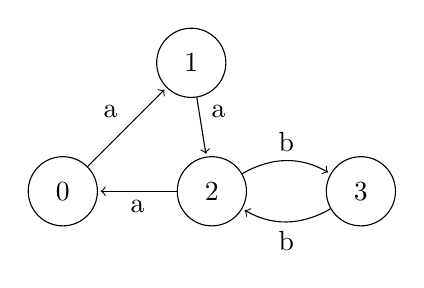
\begin{tikzpicture}[shorten >=1pt,auto]
       \node[state] (q_0)                      {$0$};
       \node[state] (q_1) [above right=of q_0] {$1$};
       \node[state] (q_2) [right=of q_0]       {$2$};
       \node[state] (q_3) [right=of q_2]       {$3$};
        \path[->]
        (q_0) edge  node {a} (q_1)
        (q_1) edge  node {a} (q_2)
        (q_2) edge  node {a} (q_0)
        (q_2) edge[bend left, above]  node {b} (q_3)
        (q_3) edge[bend left, below]  node {b} (q_2);
    \end{tikzpicture}
    \caption{The example of input graph $\mathcal{G}$}
    \label{fig:example_input_graph}
\end{figure}

We use adjacency matrix decomposed to a set of a boolean matrix as a representation of the graph.
\begin{definition}
An adjacency matrix $M$ of the graph $\mathcal{G}=$ is a square $|V|\times|V|$ matrix, such that $M[i,j] = \{l \mid e = (i,l,j) \in E\}$.
\end{definition}

Adjacency matrix $M$ of the graph $\mathcal{G}$ is

$$
    M =
    \begin{pmatrix}
    . & \{a\} & . & .     \\
    . & . & \{a\} & .     \\
    \{a\} & . & . & \{b\} \\
    . & . & \{b\} & .
    \end{pmatrix}.
$$

\begin{definition}

Boolean decomposition of adjacency matrix $M$ of graph $\mathcal{G}=$ is set of Boolean matrix $$\mathcal{M} = \{M^l \mid l \in L, M^l[i,j]=1 \iff l \in M[i,j]\}.$$

\end{definition}

Matrix $M$ can be represented as a set of two Boolean matrices $M^a$ and $M^b$ where
\begin{align}
M^{a} =
\begin{pmatrix}
    . & 1 & . & .   \\
    . & . & 1 & .   \\
    1 & . & . & .   \\
    . & . & . & .  
\end{pmatrix}, 
M^{b} =
\begin{pmatrix}      
    . & . & . & .   \\
    . & . & . & .   \\
    . & . & . & 1   \\
    . & . & 1 & . 
\end{pmatrix} \label{eq:boolean_decomposition_of_graph}
\end{align}
\subsection{Languages}

\begin{definition}\emph{Context-free grammar} is a 4-tuple $G=(N, \Sigma, R, S)$, where 
\begin{itemize}
    \item $N$ is a set of nonterminals
    \item $\Sigma$ is a set of terminals
    \item $R$ is a finite set of productions of the followings form: $A \to \alpha, ~A \in N,~ \alpha \in (N \cup \Sigma)^*$
    \item $S$ - a starting nonterminal
\end{itemize}
\end{definition}

\begin{definition} \emph{Context-free language} is a language generated by a context-free grammar:
\begin{align*}
     L(G) = \{w \in \Sigma^* \mid S \Rightarrow^* w \} 
\end{align*}
Where $S \Rightarrow^* w$  denotes that a string $w$ can be generated from a starting non-terminal $S$ using some sequence of production rules from $P$.
\end{definition}

\begin{definition} Context-free grammar $G = (N, \Sigma, R, S)$ is said to be in \emph{Chomsky normal form} if all productions in $R$ are of the form:
    \begin{itemize}
        \item $A \rightarrow BC,~A,~B,~C \in N$
        \item  $A \rightarrow a,~A \in N,~a \in \Sigma$
        \item $S \rightarrow \varepsilon,~\varepsilon$ is an empty string
    \end{itemize}
\end{definition}
Note that every context-free grammar can be transformed into an equivalent one in Chomsky Normal Form. 
\begin{definition} Context-free grammar $G = (N, \Sigma, P, S)$ is said to be in \emph{Weak Chomsky normal form} if all productions in $P$ are of the form:
    \begin{itemize}
        \item $A \rightarrow BC,~A,~B,~C \in N$
        \item  $A \rightarrow a,~A \in N,~a \in \Sigma$
        \item $A \rightarrow \varepsilon,~A \in N$
    \end{itemize}
\end{definition}
In other words, weak Chomsky normal form differs from Chomsky normal Form in the followings:
\begin{itemize}
    \item $\varepsilon$ can be derived from any non-terminal
    \item $S$ can be at a right part of productions
\end{itemize}
    
    
For example, let's consider the following context-free grammar, which generates the language $L(G) = \{A^nB^n, n \in \mathbb{N}\}$:
$G=(N, \Sigma, P, S), ~N=\{S\},~\Sigma=\{A,B\}$ and productions: 
\begin{align*}
S \rightarrow AB \\
S \rightarrow ASB\\
S \rightarrow \varepsilon
\end{align*}
After transformation to Chomsky Normal Form the resulting grammar:
\begin{align*}
S \rightarrow AB \\
S \rightarrow AC \\
C \rightarrow SB \\
S \rightarrow \varepsilon
\end{align*}

This productions itself are the grammar that has the same result as original grammar.

We use a context-free grammar in the weak Chomsky Normal Form without a starting non-terminal, which will be specified in the path queries for the graph. It should be noted that we omit the rules of the form $A \rightarrow \varepsilon$ for the reason that they correspond to trivial paths, which are more convenient to consider separately.

\begin{definition}\emph{Context-free relation} is a relation $R_A \subseteq V \times V$ for graph $G = (V, E)$, context-free grammar $G = (N,~\Sigma,~P)$ and fixed non-terminal $A$:
\begin{align*}
     R_A = \{(n, m) \mid \exists n \pi m~(l(\pi) \in L(G_A))\}
\end{align*}
\end{definition}

 Now, the definition for \emph{multiple-source (single-source) context-free path querying problem} can be formulated in the introduced notation as follows. For the given graph $G = (V, E)$, context-free grammar $G=(N, \Sigma, P)$ and set of source vertices $Src$ we need to find all context-free relations $R_A$ for any $A \in Src$. 
 
\subsection{Matrix-Based Algorithm}
Let $D = (V, E)$ be the input graph and $G = (N, \Sigma, P)$ be the input grammar. For the context-free path query evaluation, we need to provide context-free relations \mbox{$R_A \subseteq V \times V$} for every \mbox{$A \in N$}.
The matrix-based algorithm for CFPQ can be expressed in terms of operations over Boolean matrices (see listing~\ref{alg:algo0}) which is an advantage for implementation.
{\footnotesize
\begin{algorithm}
\begin{algorithmic}[1]
\caption{Context-free path querying algorithm}
\label{alg:algo0}
\Function{evalCFPQ}{$D=(V,E), G=(N,\Sigma,P)$}
    \State{$n \gets$ |V|}
    \State{$T \gets \{T^{A_i} \mid A_i \in N, T^{A_i}$ is a matrix $n \times n$, $T^{A_i}_{k,l} \gets$ \texttt{false}\} }
    \ForAll{$(i,x,j) \in E$, $A_k \mid A_k \to x \in P$}
        %\Comment{Matrices initialization}
        %\For{$A_k \mid A_k \to x \in P$}
          {$T^{A_k}_{i,j} \gets \texttt{true}$}
        %\EndFor
    \EndFor
    \ForAll{$A_k \mid A_k \to \varepsilon \in P$}
        \ForAll{$i \in \{0,\ldots ,n-1\}$}
            {$T^{A_k}_{i,i} \gets \texttt{true}$}
        \EndFor
    \EndFor

    \While{any matrix in $T$ is changing}
        %\Comment{Transitive c	losure calculation}
        \For{$A_i \to A_j A_k \in P$}
          { $T^{A_i} \gets T^{A_i} + (T^{A_j} \times T^{A_k})$ } 
        \EndFor
    \EndWhile
\State \Return $T$
\EndFunction
\end{algorithmic}
\end{algorithm}
}

This CFPQ algorithm allows efficiently apply GPGPU techniques, but it solves all-pairs problem and takes unreasonable amount of memory in scenarios in which we want to find paths from a relatively small set of vertices, since it calculates a lot of redundant information.  
\section{Matrix-based Algorithm for CFPQ}

Formal description of matrix-based algorithm.

\section{Matrix-based CFPQ for Single-Path Semantics}
In this section, we propose the matrix-based algorithm for CFPQ w.r.t. the single-path query semantics (see listing~\ref{lst:algo2}). This algorithm constructs the set of matrices $T$ with PathIndexes as elements.
{\small
	\begin{algorithm}
		\floatname{algorithm}{Listing}
		\begin{algorithmic}[1]
			\caption{CFPQ algorithm w.r.t. single-path query semantics}
			\label{lst:algo2}
			\Function{evalCFPQ}{$D=(V,E), G=(N,\Sigma,P)$}
			\State{$n \gets$ |V|}
			\State{$T \gets \{T^{A_i} \mid A_i \in N, T^{A_i}$ is a matrix $n \times n$, $T^{A_i}_{k,l} \gets \bot$ \} }
			\ForAll{$(i,x,j) \in E$, $A_k \mid A_k \to x \in P$}
			%\Comment{Matrices initialization}
			%\For{$A_k \mid A_k \to x \in P$}
			{$T^{A_k}_{i,j} \gets (i,j,i,1,1)$}
			%\EndFor
			\EndFor
			\For{$A_k \mid A_k \to \varepsilon \in P$}
			{$T^{A_k}_{i,i} \gets (i,i,i,1,0)$}
			\EndFor
			
			\While{any matrix in $T$ is changing}
			%\Comment{Transitive closure calculation}
			\For{$A_i \to A_j A_k \in P$}
			{ $T^{A_i} \gets T^{A_i} + (T^{A_j} \odot T^{A_k})$ } 
			\EndFor
			\EndWhile
			\State \Return $T$
			\EndFunction
		\end{algorithmic}
	\end{algorithm}
}

After constructing the set of matrices $T$ for every node pair $i, j$ and nonterminal $A$ we can extract a path $i \pi j$ from $i$ to $j$ such that $A \xRightarrow[G]{*} l(\pi)$ if such path exists. We also propose the algorithm (see listing~\ref{lst:algo3}) for extracting one of those paths which forms a string with minimal height of derivation tree. Our algorithm returns the empty path $[]$ only if $i = j$ and $A \to \varepsilon \in P$. Note that if the PathIndex for given $i,j,A$ is equal to $\bot$ then our algorithm returns a special path $\pi_{\emptyset}$ to denote that such a path does not exist.

{\small
	\begin{algorithm}
		\floatname{algorithm}{Listing}
		\begin{algorithmic}[1]
			\caption{Path extraction algorithm}
			\label{lst:algo3}
			\Function{extractPath}{$i, j, A, T=\{T^{A_i}\}, G=(N,\Sigma,P)$}
			\State{$index \gets T^{A}_{i,j}$ }
			
			\If{$index = \bot$}
			\State \Return $\pi_{\emptyset}$
			\Comment{Such a path does not exist}
			\EndIf
			
			\If{$index.height = 1$}
			\If{$index.length = 0$}
			\State \Return $[]$
			\Comment{Return an empty path}
			\EndIf
			\ForAll{$ x \mid (i,x,j) \in E$}
			\If{$A \to x \in P$}
			\State \Return $[(i,x,j)]$
			\Comment{Return a path of length one}
			\EndIf
			\EndFor
			\EndIf
			
			\ForAll{$A \to B C \in P$}
			\State{$index_B \gets T^{B}_{i,index.middle}$ }
			\State{$index_C \gets T^{C}_{index.middle,j}$ }			
			\If{$(index_B \neq \bot) \wedge (index_C \neq \bot)$}
			\State{$maxH \gets max(index_B.height, index_C.height)$ }
			\If{$index.height = maxH + 1$}
			
						
			\State{$\pi_1 \gets$ \Call{extractPath}{$i, index.middle, B, T, G$}}
			\State{$\pi_2 \gets$ \Call{extractPath}{$index.middle, j, C, T, G$}}
			\State \Return $\pi_1 + \pi_2$
			\Comment{Return the concatenation of paths}
			\EndIf
			\EndIf
			\EndFor
			\EndFunction
		\end{algorithmic}
	\end{algorithm}
}

\subsection{Correctness}

Let $T^{(p)} = \{T^{(p), A_i}\}$ be a constructed matrix $T$ by the algorithm in listing~\ref{lst:algo2} after $p-1$ loop iterations for $p \geq 2$, and $T^{(1)} = \{T^{(1), A_i}\}$ be a constructed matrix $T$ by this algorithm after initialization in lines 3-5. Note that the matrix $T$ returned by this algorithm is equal to $\sum_{p = 1}^{\infty} T^{(p)}$. Then the following lemma and theorem hold.

\begin{lemma}\label{lemma:correctness}
	Let $D = (V,E)$ be a graph, let $G =(N,\Sigma,P)$ be a grammar. Then for any $i, j$ and for any non-terminal $A \in N$, $index = T^{(p),A}_{i,j}$ and $index = (i,j,k,h,l) \neq \bot$ iff $(i,j) \in R_A$ and $i \pi j$, such that there is a derivation tree of the minimal height $h \leq p$ for the string $l(\pi)$  of length $l$ and a context-free grammar $G_A = (N,\Sigma,P,A)$.
\end{lemma}
\begin{proof}(Proof by Induction)
	
	\textbf{Base case}: Show that the lemma holds for $p = 1$. For any $i, j$ and for any non-terminal $A \in N$, $(i,j,k,h,l) = T^{(1), A}_{i,j}$ iff there is either $i \pi j$ of length $1$ that consists of a unique edge $e$ from the node $i$ to the node $j$ and $(A \rightarrow x) \in P$, where $x = l(\pi)$, or $i = j$ and $(A \rightarrow \varepsilon) \in P$, where $\varepsilon = l(\pi)$. Therefore $(i,j) \in R_A$ and there is a derivation tree of the minimal height $h = p = 1$, shown on Figure~\ref{tree1}, for the string $x$ and a context-free grammar $G_A = (N,\Sigma,P,A)$. Thus, it has been shown that the lemma holds for $p = 1$.
	
	\begin{figure}[h!]
		\centering
		\includegraphics[width=2cm]{pictures/tree1.pdf}
		\caption{The derivation tree of the minimal height $p = 1$ for the string $x = l(\pi)$ where $x \in \Sigma \cup \{\varepsilon\}$.}
		\label{tree1}
	\end{figure}
	
	\textbf{Inductive step}: Assume that the lemma holds for any $p \leq (q - 1)$ and show that it also holds for $p = q$, where $q \geq 2$.
	
	The index $(i,j,k,h,l) = T^{(q),A}_{i,j}$ iff there is exists a rule $(A \to B C) \in P$ such that $(i,j,k,h,l) = M_{i,j}$ where $$M = T^{(q-1),A} + (T^{(q-1),B} \odot T^{(q-1),C}).$$ 
	
	Let $(i,j,k,h,l) = T^{(q-1),A}_{i,j}$. By the inductive hypothesis, $(i,j,k,h,l) = T^{(q-1),A}_{i,j}$ iff $(i,j) \in R_A$ and there exists $i \pi j$, such that there is a derivation tree of the minimal height $h \leq (q-1)$ for the string $l(\pi)$ and a context-free grammar $G_A = (N,\Sigma,P,A)$. The statement of the lemma holds for $p = q$ since the height $h$ of this tree is also less than or equal to $q$.
	
	Now, let $(i,j,k,h,l) = (T^{(q-1),B} \odot T^{(q-1),C})_{i,j}$. By the definition of the binary operation $\odot$, $(i,j,k,h,l) = (T^{(q-1),B} \odot T^{(q-1),C})_{i,j}$ iff there are $r=k$, $(i,r,\_,h_1,l_1) = T^{(q-1),B}_{i,r}$ and $(r,j,\_,h_2,l_2) = T^{(q-1),C}_{r,j}$, such that $q = max(h_1, h_2) + 1$, $l = l_1 + l_2$. Hence, by the inductive hypothesis, there are $i \pi_1 r$ and $r \pi_2 j$, such that $(i,r) \in R_B$ and $(r,j) \in R_C$, and there are the derivation trees $T_B$ and $T_C$ of minimal heights $h_1 \leq (q-1)$ and $h_2 \leq (p-1)$ for the strings $w_1 = l(\pi_1)$, $w_2 = l(\pi_2)$ and the context-free grammars $G_B$, $G_C$ respectively. Thus, the concatenation of paths $\pi_1$ and $\pi_2$ is $i \pi j$, where $(i,j) \in R_A$ and there is a derivation tree of the minimal height $h = 1 + max(h_1, h_2)$, shown on Figure~\ref{tree2}, for the string $w = l(\pi)$ of length $l = l_1 + l_2$ and a grammar $G_A$.
	\begin{figure}[h!]
		\centering
		\includegraphics[width=5cm]{pictures/tree2.pdf}
		\caption{The derivation tree of the minimal height $h = 1 + max(h_1, h_2)$ for the string $w = l(\pi)$, where $T_B$ and $T_C$ are the derivation trees for strings $w_1$ and $w_2$ respectively.}
		\label{tree2}
	\end{figure}
	
	The statement of the lemma holds for $p = q$ since the minimal height $h = 1 + max(h_1, h_2) \leq q$. This completes the proof of the lemma.
\end{proof}

\begin{mytheorem}\label{thm:correct}
	Let $D = (V,E)$ be a graph and let $G =(N,\Sigma,P)$ be a grammar. Then for any $i, j$ and for any non-terminal $A \in N$, $index = T^A_{i,j}$ and $index = (i,j,k,h,l) \neq \bot$ iff $(i,j) \in R_A$ and $i \pi j$, such that there is a derivation tree of the minimal height $h$ for the string $l(\pi)$ of length $l$ and a context-free grammar $G_A = (N,\Sigma,P,A)$.
\end{mytheorem}
\begin{proof}
	
	Since the matrix $T = \sum_{p = 1}^{\infty} T^{(p)}$ for any $i, j$ and for any non-terminal $A \in N$, $index = T^A_{i,j}$ and $index = (i,j,k,h,l) \neq \bot$ iff there is $p \geq 1$, such that $index \in T^{(p),A}_{i,j}$. By the lemma~\ref{lemma:correctness}, $index = T^{(p),A}_{i,j}$ iff $(i,j) \in R_A$ and $i \pi j$, such that there is a derivation tree of the minimal height $h \leq p$ for the string $l(\pi)$  of length $l$ and a context-free grammar $G_A = (N,\Sigma,P,A)$. This completes the proof of the theorem.
\end{proof}

Now, using the theorem~\ref{thm:correct} and induction on the length of the path, it can be easily shown that the following theorem holds.

\begin{mytheorem}\label{thm:correct_extraction}
	Let $D = (V,E)$ be a graph, let $G =(N,\Sigma,P)$ be a grammar and $T$ be a set of matrices returned by the algorithm in listing~\ref{lst:algo2}. Then for any $i, j$ and for any non-terminal $A \in N$ such that $index = T^A_{i,j}$ and $index = (i,j,k,h,l) \neq \bot$, the algorithm in listing~\ref{lst:algo3} for these parameters will return a path $i \pi j$ such that $(i,j) \in R_A$ and there is a derivation tree of the minimal height $h$ for the string $l(\pi)$ of length $l$ and a context-free grammar $G_A = (N,\Sigma,P,A)$.
\end{mytheorem}

We can, therefore, determine whether $(i,j) \in R_A$ by asking whether $T^A_{i,j} = \bot$. Also, we can extract such a path which forms a string with a derivation tree of minimal height by using our algorithm in listing~\ref{lst:algo3}. Thus, we show how the context-free path query evaluation w.r.t. the single-path semantics can be solved in terms of matrix operations.

\subsection{Complexity}

Denote the number of elementary operations executed by the algorithm of multiplying two $n \times n$ matrices with PathIndexes as $MM(n)$. Also, denote the number of elementary operations, executed by the matrix element-wise + operation of two $n \times n$ matrices with PathIndexes as $MA(n)$. Since the line \textbf{7} of the algorithm in listing~\ref{lst:algo2} is executed no more than $|V|^2|N|$ times, the following theorem holds.

\begin{mytheorem}\label{thm:time}
	Let $D = (V,E)$ be a graph and let $G =(N,\Sigma,P)$ be a grammar. The algorithm in listing~\ref{lst:algo2} calculates the set of matrices $T$ in $O(|V|^2|N|^3(MM(|V|) + MA(|V|)))$.
\end{mytheorem}

Also, denote the time complexity of the access to the PathIndex in the $n \times n$ matrix as $Access(n)$. Then the following theorem on the time complexity of the path extraction algorithm holds.

\begin{mytheorem}\label{thm:time_extraction}
	Let $D = (V,E)$ be a graph, let $G =(N,\Sigma,P)$ be a grammar and $T$ be a set of matrices returned by the algorithm in listing~\ref{lst:algo2}. Then for any $i, j$ and for any non-terminal $A \in N$ such that $index = T^A_{i,j}$ and $index = (i,j,k,h,l) \neq \bot$, the algorithm in listing~\ref{lst:algo3} for these parameters calculates a path $i \pi j$ in $O(l \times N \times Access(|V|))$.
\end{mytheorem}

\subsection{An Example}
In this section, we provide a step-by-step demonstration of the proposed algorithms. For this, we consider the example with the worst-case time complexity.

The \textbf{example query} is based on the context-free grammar $G = (N, \Sigma, P)$ of the worst-case example query where:
\begin{itemize}
	\item the set of non-terminals $N = \{S\}$;
	\item the set of terminals $\Sigma = \{a, b\}$;
	\item the set of production rules $P$ is presented on Figure~\ref{ProductionRulesWorsCaseExample}.
\end{itemize}

\begin{figure}[h]
	\[
	\begin{array}{rccl}
	0: & S & \rightarrow & \text{\emph{a}} \ S \ \text{\emph{b}} \\
	1: & S & \rightarrow & \text{\emph{a}} \ \text{\emph{b}} \\ 
	\end{array}
	\]
	\caption{Production rules for the worst-case example.}
	\label{ProductionRulesWorsCaseExample}
\end{figure}

Since the proposed algorithm processes only grammars in Chomsky normal form, we first transform the grammar $G$ into an equivalent grammar $G' = (N', \Sigma', P')$ in normal form, where:
\begin{itemize}
	\item the set of non-terminals $N' = \{S, S_1, A, B\}$;
	\item the set of terminals $\Sigma' = \{a, b\}$;
	\item the set of production rules $P'$ is presented on Figure~\ref{ProductionRulesExampleQueryCNF}.
\end{itemize}

\begin{figure}[h]
	\[
	\begin{array}{rccl}
	0: & S & \rightarrow & A \ B \\
	1: & S & \rightarrow & A \ S_1 \\
	2: & S_1 & \rightarrow & S \ B \\
	3: & A & \rightarrow & \text{\emph{a}} \\ 
	4: & B & \rightarrow & \text{\emph{b}} \\ 
	\end{array}
	\]
	\caption{Production rules for the example query grammar in normal form.}
	\label{ProductionRulesExampleQueryCNF}
\end{figure}

We run the query on a graph, presented in Figure~\ref{Example_Graph}. We provide a step-by-step demonstration of the work with the given graph $D$ and grammar $G'$ of the algorithm in listing~\ref{lst:algo2}. After the matrix initialization in lines \textbf{3-5} of this algorithm, we have a matrix $T^{(1)}$, presented on Figure~\ref{ExampleQueryInitMatrix}.

\begin{figure}[h]
	\[
	T^{(1),A} = \begin{pmatrix}
	\bot & (0,1,0,1,1)       & \bot & \bot       \\
	\bot & \bot & (1,2,1,1,1)       & \bot \\
	(2,0,2,1,1)       & \bot & \bot & \bot \\
	\bot       & \bot & \bot & \bot \\
	\end{pmatrix}
	\]
	\[
	T^{(1),B} = \begin{pmatrix}
	\bot & \{A\}       & \bot & (0,3,0,1,1)       \\
	\bot & \bot & \{A\}       & \bot \\
	\{A\}       & \bot & \bot & \bot \\
	(3,0,3,1,1)      & \bot & \bot & \bot \\
	\end{pmatrix}
	\]
	\caption{The initial matrix for the example query. The PathIndexes $T^{(1),S_1}_{i,j}$ and $T^{(1),S}_{i,j}$ are equal to $\bot$ for every $i,j$.}
	\label{ExampleQueryInitMatrix}
\end{figure}

After the initialization, the only matrices which will be updated are $T^{S_1}$ and $T^{S}$. These matrices obtained after the first loop iteration is shown in Figure~\ref{ExampleQueryFirstIteration}.

\begin{figure}[h]
	\[
	T^{(2),S} = \begin{pmatrix}
	\bot & \bot       & \bot & \bot       \\
	\bot & \bot & \bot       & \bot \\
	\bot       & \bot & \bot & (2,3,0,2,2) \\
	\bot       & \bot & \bot & \bot \\
	\end{pmatrix}
	\]
	\caption{The first iteration of computing the transitive closure for the example query. The PathIndexes $T^{(1),S_1}_{i,j}$ are equal to $\bot$ for every $i,j$.}
	\label{ExampleQueryFirstIteration}
\end{figure}

When the algorithm at some iteration finds new paths for some nonterminal in the graph $D$, then it adds corresponding PathIndexes to the matrix for this nonterminal. For example, after the first loop iteration, PathIndex $(2,3,0,2,2)$ is added to the matrix $T^{S}$. This PathIndex is added to the element with a row index $i = 2$ and a column index $j = 3$. This means, that there is $i\pi j$ (a path $\pi$ from the node 2 to the node 3), such that $S \xRightarrow[G]{*} l(\pi)$, this path obtained by concatenation of smaller paths via node 0, the length of the path is equal to 2, and the derivation tree for the string $l(pi)$ has a height 2.

The calculation of the transitive closure is completed after $k$ iterations, when a fixpoint is reached: $T^{(k)} = T^{(k+1)}$. For the example query, $k = 13$ since $T_{13} = T_{14}$. The resulted matrices are presented on Figure~\ref{ExampleQueryFinalMatrices}.

\begin{figure}[h]
	\[
	T^{(14),S} = \begin{pmatrix}
	(0,0,1,12,12) & \bot       & \bot & (0,3,1,6,6)       \\
	(1,0,2,4,4) & \bot & \bot       & (1,3,2,10,10) \\
	(2,0,0,8,8)       & \bot & \bot & (2,3,0,2,2) \\
	\bot       & \bot & \bot & \bot \\
	\end{pmatrix}
	\]
	
	\[
	T^{(14),S_1} = \begin{pmatrix}
	(0,0,3,7,7)  & \bot       & \bot & (0,3,0,13,13)       \\
	(1,0,3,11,11) & \bot & \bot       & (1,3,0,5,5) \\
	(2,0,3,3,3)       & \bot & \bot & (2,3,0,9,9) \\
	\bot       & \bot & \bot & \bot \\
	\end{pmatrix}
	\]
	\caption{The final matrices after computing the transitive closure for the example query.}
	\label{ExampleQueryFinalMatrices}
\end{figure}

Thus, the result of the algorithm in listing~\ref{lst:algo2} for the example query are the matrices on Figures~\ref{ExampleQueryInitMatrix} and \ref{ExampleQueryFinalMatrices}. Now, after constructing the transitive closure, we can construct the context-free relations $R_A$. These relations for each non-terminal of the grammar $G'$ are presented on Figure~\ref{ExampleQueryCFRelations}.

\begin{figure}[h]
	\begin{eqnarray*}
		R_S&=&\{(0,0),(0,3),(1,0),(1,3),(2,0),(2,3)\},\\
		R_{S_1}&=&\{(0,0),(0,3),(1,0),(1,3),(2,0),(2,3)\},\\
		R_{A}&=&\{(0,1),(1,2),(2,0)\}, \\
		R_{B}&=&\{(0,3), (3,0)\}.
	\end{eqnarray*}
	\caption{Context-free relations for the example query.}
	\label{ExampleQueryCFRelations}
\end{figure}

In the context-free relation $R_S$, we have all node pairs corresponding to paths, whose labeling is in the language $L(G_S) = \{a^n b^n| n \geq 1\}$. Using the algortihm in listing~\ref{lst:algo3} we can restore paths for each node pair from context-free relations. For example, given $i=j=0$, nonterminal $S$, set of resulted matrices $T$, and context-free grammar $G'$, the algorithm in listing~\ref{lst:algo3} returns a path $0\pi 0$ whose labeling forms a string $l(\pi) = a^6 b^6$. The length of path $\pi$ is equal to 12 and the height of the derivation tree for $l(\pi)$ is equal to 12, which is consistent with the corresponding PathIndex $T^{(14),S}_{0,0}$.
\subsection{Архитектура решения}
\paragraph{}

Архитектура предлагаемого решение приведена на рисунке \ref{fig:arch}.
\begin{figure}[h!]
\centering
\includegraphics[scale=0.5]{pictures/dia3.png}
\caption{Архитектура предлагаемой библиотеки GraphBLAS-sharp}
\label{fig:arch}
\end{figure}

В рамках данной работы были реализованы компоненты библиотеки GraphBLAS-sharp, описанные ниже.
\begin{itemize}
    \item \textbf{Модули коллекций Matrix и Vector}. Модули содержат абстрактные классы для представления матрицы и вектора, реализованные в виде размеченного объединения, а также конкретные форматы их хранения.
    \item \textbf{Модули операций Matrix и Vector}. Модули содержат определение операций стандарта GraphBLAS для работы с абстрактными коллекциями.
    \item \textbf{Модуль AlgebraicStructures}. Модуль содержит реализацию не\-ко\-то\-рых алгебраических структур, таких как моноид и полукольцо.
    \item \textbf{Модуль Predefined}. Модуль содержит реализацию представителей классов алгебраических структур для встроенных типов данных. Так, например, в модуле реализованно стандартное булево полукольцо, стандартное арифметическое полукольцо над встроенными типами данных, а также тропическое полукольцо.
    \item \textbf{Модуль GraphblasEvaluation}. Модуль содержит вычислительное выражение GraphblasEvaluation. Оно выполняет 2 функции --- во-первых, являясь по своей сути монадой Reader, позволяет выставлять глобальные и локальные параметры вычисления, а во-вторых, оно скрывает использование интерфейса для работы с OpenCL, который предоставляет библиотека Brahma.Fsharp.
    \item \textbf{Модуль MtxReader}. Модуль предназначен для импорта матриц из файлов в формате \textit{mtx}.
    \item \textbf{Модуль Algorithms}. Модуль содержит небольшой набор классических алгоритмов на графах. В нем реализованы следующие алгоритмы: 
    \begin{itemize}
        \item алгоритм поиска в ширину из единственной вершины
        \item алгоритм поиска кратчайшего пути из единственной вершины
        \item алгоритм подсчета числа треугольников в графе
        \item алгоритм вычисления меры центральности вершины
    \end{itemize}
    \item \textbf{Модуль Backend}. Модуль содержит реализацию соответствующих операций для конкретных форматов хранения матрицы и вектора. В рамках данной работы были реализованны следующие операции:
    \begin{itemize}
        \item умножение матрицы в CSR формате на разреженный вектор
        \item транспонирование матрицы в CSR формате
        \item создание разреженного вектора из списка элементов
    \end{itemize}
\end{itemize}

\subsection{Реализация коллекций}
\paragraph{}
Особенностью стандарта GraphBLAS является то, что описываемые в нем объекты абстрактны --- за реализацию внутреннего хранения объектов ответственен разработчик решения. 

В качестве форматов хранения матрицы используются 2 формата --- CSR и COO.
Матрицы, которые выражают графы, обычно сильно разреженны, поэтому использовать плотную матрицу в качестве внутренней реализации нецелесообразно.
CSR формат, по сравнению, например, с диагональным (DIA) или ELLPACK (ELL) форматом, лучше подходит для хранения произвольных разреженных матриц, так как не требует от матрицы соответствия определенному паттерну для эффективного хранения. По сравнению с COO он занимает $2 \cdot nnz + n + 1$ вместо $3\cdot nnz$ памяти (здесь и далее $nnz$ --- число ненулевых элементов матрицы, $n$ --- число строк матрицы, $m$ --- число столбцов) и предоставляет доступ к произвольной строке за $O(1)$, что является существенным преимущество при реализации параллельных алгоритмов. В то же время для хранения сверхразреженных матриц, у которых $nnz > (m\cdot(n-1)-1)/2$ лучше подходит формат COO.

\subsection{Реализация операций}
\subsubsection{Умножение матрицы в CSR формате на разреженный вектор}
\paragraph{}
Для реализации операции умножения матрицы на вектор были рассмотрены несколько алгоритмов. В статье за авторством W. Liu and B. Vinter\cite{esc} приводится алгоритм умножения разреженных матриц в CSR формате. Ключевой операцией в алгоритмах такого рода является операция слияния строк промежуточной матрицы. Так как все строки имеют разное число ненулевых элементов, то для данной операции особо важно выбрать эффективный метод балансирования нагрузки. В данной статье предлагается разделить все строки промежуточной матрицы на 38 групп в зависимости числа ненулевых элементов в них и для каждой группы использовать один из четырех алгоритмов слияния. Однако, как показывает последние работы в данной области\cite{hash}, существуют более производительные и простые в решения. Так, статья за авторством Y. Nagasaka и др.\cite{hash}, которая также описывает алгоритм умножения разреженных матриц в CSR формате, предлагает для слияния строк использовать хеш-таблицу. По словам автора, этот алгоритм выигрывает у предыдущего и по времени работы, и по количеству потребляемой памяти. Однако для обновления данных в хеш-таблице алгоритм использует атомарные операции, а атомарные операции над произвольными типами на данный момент не поддерживаются библиотекой Brahma.FSharp, поэтому реализовать данный алгоритм оказалось невозможно. Алгоритм, описывающий умножение матрицы в CSR формате на разреженный вектор, за авторством Y. Tao и др.\cite{atomic} также предполагает использование атомарных операций, что делает невозможным его реализацию. Другой метод авторов Yang, C., Wang, Y., и Owens, J. D\cite{mxv_bfs} описывает умножения матрицы в CSR формате на разреженный вектор в контексте применения его в алгоритмах, подобных алгоритму поиска в ширину, а при оценке эффективности работы использует допущение о том, что вектор имеет небольшое число ненулевых элементов. Несмотря на то, что именно этот алгоритм реализован в аналогичной библиотеке GraphBLAST, было решено отказаться от него в пользу альтернативного варианта. В предлагаемой работе был реализован следующий алгоритм.
\begin{enumerate}
    \item Каждая строка матрицы умножается на разреженный вектор.
    \begin{itemize}
        \item Каждая строка обрабатывается 1 рабочей группой.
        \item Каждый поток в рабочей группе обрабатывает 1 элемент левого вектора с шагом, равным размеру рабочей группы.
        \item Значение с нужным индексом в правом векторе ищется бинарным поиском.
    \end{itemize}
    \item Полученный вектор промежуточных значений фильтруется от нулевых элементов с использованием префиксной суммы.
\end{enumerate}

\subsubsection{Транспонирование матрицы в CSR формате}
\paragraph{}
Для транспонирования матрицы в CSR формате был реализован наивный алгоритм, предполагающий конвертацию матрицы в формат COO.
\begin{enumerate}
    \item Матрица в CSR формате конвертируется в формат COO.
    \item Индексы элементов сортируются битонической сортировкой так, чтобы соответствовать транспонированной матрице.
    \item Матрица в COO формате конвертируется обратно в формат CSR.
\end{enumerate}

\subsection{Тестирование и непрерывная интеграция}
\paragraph{}
Использование высокоуровневого языка для реализации стандарта GraphBLAS, в том числе, облегчает тестирование. В GraphBLAS внутреннее поведение операции зависит от объектов управления и от того, как именно реализованы абстрактные объекты коллекций, причем с ростом числа используемых реализаций число вариантов операции, которые нужно тестировать, растет экспоненциально. В реализациях на С++, в которых для тестирования применялся Boost Test Framework, отдельно тестируется каждый вариант и, как правило, только на одном типе данных. 

В данной работе для тестирования используется библиотека Expecto\footnote{Репозиторий библиотеки Expecto: \url{https://github.com/haf/expecto}. Дата посещения: 01.06.2021}. За счет интеграции с библиотекой FsCheck\footnote{Репозиторий библиотеки FsCheck: \url{https://github.com/fscheck/FsCheck}. Дата посещения: 01.06.2021}, она поддерживает property-based тестирование, что позволяет автоматически генерировать наборы данных для тестов. Кроме того, она позволяет писать комбинаторные параметрические тесты, благодаря чему можно легко проверить все возможные варианты операции.

Возможность исполнения на CPU программ, которые используют OpenCL, позволила легко настроить тестирование библиотеки в сервисах непрерывной интеграции, таких как AppVeyor и GitHub Actions. 
\section{Dataset description}

In our evaluation we use \textbf{[RDF]} dataset which contains the following parts.
\begin{itemize}
\item The real-world data RDFs provided in CFPQ\_Data dataset\footnote{CFPQ\_Data dataset GitHub repository: \url{https://github.com/JetBrains-Research/CFPQ_Data}. Access date: 12.11.2019.} from~\cite{Mishin:2019:ECP:3327964.3328503}.
\item Geospecies (RDF which contains information about biological hierrarchy\footnote{\url{https://old.datahub.io/dataset/geospecies}. Access date: 12.11.2019.} and same generation query over \textit{broaderTransitive} relation) is provided in~\cite{Kuijpers:2019:ESC:3335783.3335791} and integrated in our evaluation with CFPQ\_Data.
\item It was shown in~\cite{Mishin:2019:ECP:3327964.3328503} that matrix-based algorithm is performant enough to handle bigger RDFs than those used in the initial datasets, such as~\cite{RDF}.
So, we add a number of big RDFs to CFPQ\_Data and use them in our evaluation.
New RDFs: \textit{go-hierarchy, go, enzime, core, pathways} are from UniProt database\footnote{Protein sequences data base: \url{https://www.uniprot.org/}. RDFs with data are avalable here: \url{ftp://ftp.uniprot.org/pub/databases/uniprot/current_release/rdf}. Access date: 12.11.2019}, and \textit{eclass-514en} is from eClassOWL project\footnote{eClassOWL project: \url{http://www.heppnetz.de/projects/eclassowl/}. eclass-514en file is available here: \url{http://www.ebusiness-unibw.org/ontologies/eclass/5.1.4/eclass_514en.owl}. Access date: 12.11.2019.}.
\end{itemize}

The variants of the \textit{same generation query}~\cite{FndDB} are used in almost all cases because it is an important example of real-world queries that are context-free but not regular.
So, variations of the same generation query are used in our evaluation.
All queries are added to the CFPQ\_Data dataset.

We use two queries over \textit{subClassOf} and \textit{type} relations.
The first query is the grammar $G_1$:
\[
 \begin{array}{lcl}
   s  \rightarrow \textit{subClassOf}^{\ -1} \ s \ \textit{subClassOf}   & \quad & s  \rightarrow \textit{type}^{\ -1} \ s \ \textit{type}     \\
   s  \rightarrow \textit{subClassOf}^{\ -1} \ \textit{subClassOf}       & \quad & s  \rightarrow  \textit{type}^{\ -1}  \ \textit{type}

 \end{array}
 \]
The second one is the grammar $G_2$: \[s \rightarrow \textit{subClassOf}^{\ -1} \ s \ \textit{subClassOf} \mid  \textit{subClassOf}\]

For geospecies we use same-generation queries from the original paper $geo$: \[s \rightarrow \textit{broaderTransitive} \ s \ \textit{broaderTransitive}^{\ -1} \]
\[s \rightarrow \textit{broaderTransitive}  \ \textit{broaderTransitive}^{\ -1} \]


The properties of the RDFs from the dataset are given in tables \ref{tbl:propRDF} and \ref{tbl:propGeo}.

{\setlength{\tabcolsep}{0.4em}
	\begin{table*}[h]
		\caption{RDFs properties}
		\label{tbl:propRDF}
		\rowcolors{2}{}{lightgray}
		\begin{tabular}{| l | c | c | c | c |}
			\hline
			Name                  & \#V    & \#E     & \#type &\#subClassOf \\
			\hline
			\hline
			atom-primitive				& 291		& 685		& 138	& 122	\\
			univ-bench					& 179		& 413		& 84		& 36		\\
			travel						& 131		& 397		& 90		& 30		\\
			skos							& 144		& 323		& 70		& 1		\\
			people\_pets					& 337		& 834		& 161	& 33		\\
			generations					& 129		& 351		& 78		& 0		\\
			foaf							& 256		& 815		& 174	& 10		\\
			biomedical-mesure-primitive	& 341		& 711		& 130	& 122	\\
			funding						& 778		& 1480		& 304	& 90               \\
			pizza						& 671		& 2604		& 365	& 259              \\
			wine							& 733		& 2450		& 485	& 126              \\
			core							& 1323		& 8684		& 1412	& 178              \\
			pathways						& 6238		& 37196		& 3118 	& 3117             \\
			go-hierarchy					& 45007		& 1960436	& 0		& 490109           \\
			enzyme						& 48815		& 219390		& 14989	& 8163             \\
			eclass\_514en				& 239111		& 1047454	& 72517	& 90962            \\
			go							& 272770		& 1068622	& 58483	& 90512            \\
			\hline
		\end{tabular}
	\end{table*}
}


{\setlength{\tabcolsep}{0.4em}
	\begin{table*}[h]
		\caption{Geospecies properties}
		\label{tbl:propGeo}
		\rowcolors{1}{}{lightgray}
		\begin{tabular}{| c | c | c |}
			\hline
			\#V    & \#E     & \#broaderTransitive \\
			\hline
			\hline
			450609 & 2311461 & 20867 \\
			\hline
		\end{tabular}
	\end{table*}
}

\section{Evaluation}

This section describes the methodology and answers the following research questions.

\begin{enumerate}
    \item Does fusion via distillation give any benefits at the software and hardware levels?
    \item What are the properties of the generated hardware?
    \item Does the generated hardware outperform software implementations?
\end{enumerate}

\subsection{Methodology}

Our focus is on creating a basis for future research and experiments, thus we make our experiments as much reproducible as possible\footnote{\url{https://github.com/sedwards-lab/fhw/tree/sparse-linear-algebra-distillation/examples/QTreeBenchmarks/diploma/verilog-bool-no-nnz-inlined} (online; accessed:
2022-06-07) Here one could find all the results. For each benchmark all statistics are specified: matrix names, their sizes, collected metrics for both hardware and software benchmarks.}. We benchmarked the following list of chained functions. The choice is prompted by the current state of the distiller: at the moment, it does not successfully distill matrix multiplication. However, the functions are still practical enough, for example, chained addition could be seen in Luby's maximal independent set algorithm and clearly describe the applicability of the proposed approach.

\begin{itemize}
    \item \mintinline{Haskell}{mAdd (==False) (||) (mAdd (==False) (||) m1 m2) m3}
    \item \mintinline{Haskell}{mask (mAdd (== False) (||) m2 m3) (m1)}
    \item \mintinline{Haskell}{map (==Zero) (to_nat) (mAdd (==False) (||) m1 m2}
    \item \mintinline{Haskell}{map (==Zero) (to_nat) (kron (==False) (&&) m1 m2}
\end{itemize}

Above, \mintinline{Haskell}{Zero} and \texttt{to\_nat} are corresponding definitions for Peano arithmetics, since the \texttt{.pot} language does not have any primitives. For the same reason, we operated with boolean matrices. Such functions could be abstracted with free variables and then instantiated in the emitted Haskell code. However, to get maximum from distillation, we provided all the information about the functions. 

For these functions, we compared the execution time of distilled and not distilled hardware generated circuits, execution time of original and distilled Haskell code and reference \textit{Suite Sparse}\footnote{\url{https://github.com/DrTimothyAldenDavis/GraphBLAS} (online; accessed:
2022-06-07), Suite Sparse library sources.}\textsuperscript{,}\footnote{The library also uses different variations of coordinate formats (opaque to the user) and not a quadtree representation.} variants of these functions in C\texttt{++}. Note that SuiteSparse does not support recursive data types, thus only the first two function chains were implemented in SuiteSparse (since Peano number is essentially a linked list). We did not replace Peano numbers with integers, so our experiments could be interpreted easier. For hardware experiments we collected execution time and the number of memory writes and reads, to access how well fusion is performed. For software experiments we only measured the execution time. Also note that we measured only the time, required to execute the lines above, not including any IO, required to get and evaluate function arguments. But in hardware benchmarks we measured the time required to pass arguments into the circuit's memory, because such IO is inevitable. It is tricky to make such measures in Haskell due to laziness, thus the programs were compiled with \texttt{--fno-full-laziness} to turn off memoization. Also all the arguments were forced to normal form via \texttt{force} and \texttt{evaluate}. Haskell programs were compiled\footnote{GHC 8.10.4.} with \texttt{-O2 --fno-full-laziness} and Suite Sparse was compiled with default flags and linked as a shared library to C\texttt{++} code.

We took matrices from SuiteSparse matrix collection with sizes ranging from \texttt{64x64} to \texttt{512x512}. We limited ourselves with such sizes due to the fact that this is the maximum sizes that fit into \texttt{bram} with $2^{16}$ address space. Such number of \texttt{bram} blocks is available only on really expensive FPGA boards, thus in practice sizes would be smaller to achieve better utilization. Once again, it models the situation when data fits into the cache, since \texttt{bram} in our circuits will operate as a cache in real application.

\subsection{Experiments}

Table~\ref{tab:bench_results} shows the results of all execution time benchmarks. To evaluate execution time for hardware simulation, implementation stage was performed to assess the maximum frequency of FPGA device used for synthesis and implementation, and the number of execution cycles was multiplied by the number of nanoseconds a clock cycle takes. The frequencies were equal within the same benchamark set, i.e., frequency was not affected by distillation. We used \texttt{xcu250figd2104-2L} device\footnote{\url{https://www.xilinx.com/products/boards-and-kits/alveo/u250.html}  (online; accessed:
2022-06-07)} for synthesis and implementation stages. It is not really a casual and affordable chip, but it contains enough \texttt{bram} for our evaluation to see scalability. In the table a median across several benchmarks is shown. 

As it could be seen, distillation steadily increases performance: up to 2x speedup for hardware simulation and up to 3x for software benchmarks. The results are maintained within the borders of the corresponding confidence interval and the borders are not shown for brevity. Hardware speedup is lower due to the different execution semantics, dataflow is not reduction-based and distillation is a reduction-based transformation. Note that generated hardware appears to be less performant than both Haskell and C\texttt{++}, which a bit contradicts the results from~\cite{oldfhw}. For hardware benchmarks \texttt{time (IO)} shows the execution time including the time needed to transfer the data though the arguments, \texttt{time (no IO)} does not include it in its turn. It could be seen that not all the benchmarks are computationally extensive enough to cover memory transferring costs, but for more complex examples the ratio would be better. Since we basically transfer the matrices node by node from a file in the testbench, we have probably the lowest possible latency, and in practice it would be higher if reading from DDR, however the bandwidth could be increased. Noticeably, running times for \texttt{mMaskAdd} for C\texttt{++} and distilled Haskell are similar, which shows that fusion really provides some extra performance: SuiteSparse at the moment does not implement any fusion.

Table~\ref{tab:mem_results} summarizes the ratios between distilled and not distilled hardware circuits memory reads and writes. Since in general case distillation removes extra pattern matching, essentially it saves memory reads and writes. The eventual number of memory reads and writes is implementation dependent, thus the table shows what share of speedup is prompted by saving memory operations. Distillation successfully reduces the number of memory accesses, about 15\% on average. \texttt{mMapKron} has a bit higher ratio due to the fact that \texttt{Nat} numbers require additional memory accesses, since the type is recursive. It could also be seen that a major part of speedups is attributed to saved memory accesses. 

Finally, table~\ref{tab:resource_util} shows device resources utilization ratios between distilled and not distilled hardware circuits and frequencies. Columns are device primitives: registers, lookup tables, \texttt{bram} blocks or multiplexers. Utilization for both types of circuits is below 1\% of available resources on the device, except for the memory. Memory blocks utilization is about 30\% (since we choose larger \texttt{brams} to store larger matrices). Apart from that, distilled circuits could have both higher and lower utilization. Since the hardware generation is primarily syntax-directed it follows from the distilled program structure. For example, distillation might glue two recursive functions into one (in that case, memory utilization would be lower, because each cluster of mutually recursive functions possesses its own heap) or make more recursive functions than in the original program. The frequencies are the same, however, they possibly could be made better with more intelligent buffer allocation.

\subsection{Discussion}
Answering the research questions above.

\begin{enumerate}
    \item Fusion gives significant benefits, however at the hardware level the benefits are a bit smaller since hardware semantics is not reduction based. The benefits at the hardware level are mostly determined by the reduced number of memory accesses (each access takes 2 clock cycles). Notably, distilled Haskell implementation of \texttt{mMaskAdd} has similar performance with C\texttt{++}. 
    \item Device utilization is low, but such circuits could be copied on the same device to provide better utilization and higher parallelism. Resource utilization might be both better and worse after distillation, depending on the transformed program itself since translation is syntax-directed. Frequency could be increased by more intelligent buffering strategy.
    \item Although we use low-latency design with \texttt{bram}s that take 2 clock cycles per request and transfer matrices from files, which does not have any latency in simulation, we get slower execution time than Haskell and C\texttt{++} counterparts. It could be partly due to excessive buffering performed by FHW at the moment. Also there is no pipelining for recursive calls, i.e. only one set
of function argument tokens are allowed to enter a tail-recursive function call until a result is finally generated. Further CPS transformation hinders parallelization, which could be made more explicit with SSA. Some other optimizations exist that may significantly influence the performance. Also, since device utilization is about 1\%, such circuits could be copied on one device and provide more parallelism. A more detailed discussion could be found at~\cite{Edwards2019FHWP}.
\end{enumerate}

Distillation clearly showed its applicability to optimization of sparse linear algebra routines and notably it still could be combined with other techniques, like rewrite rules to achieve better results. High-level synthesis has a room for improvements by increasing pipelining, parallelism and frequency and the generated hardware could be improved from usability perspective: a support for arbitrary sized matrices is desirable. Thus we will focus on these directions. Probably a better solution would be to embed \texttt{.pot} language into e.g. Haskell to leverage its type system (to be able to use some rewrite rules as well), and add support for primitive types and parallel primitives to be able to conduct a more scalable comparison with SuiteSparse (since SuiteSparse is multithreaded). For such embedding different execution models could be implemented, including hardware synthesis, for which SSA form of GRIN looks promising, as well as extra optimizations shipped with GRIN. For hardware synthesis, an interesting direction is achieving predictable results in hardware from certain modifications in software. This property partly holds for the current approach, since the translation is syntax- directed. More information on this could be found at~\cite{predict}.

\pagebreak

\begin{table}[t]
\scriptsize
\centering
\caption*{mAddAdd}
\begin{tabular}{|c|c|c|c|c|c|c|c|c|c|} 
\hline
\rowcolor{LightBlue}
\multicolumn{3}{|c|}{Matrices dimensions} & Haskell & Haskell (distilled) & \multicolumn{2}{c|}{FHW} & \multicolumn{2}{c|}{FHW (distilled)} & {C\texttt{++}}\\
% \rowcolor{LightBlue}
\hline
m1 & m2 & m3 & time & time & time (no IO) & time (IO) & time (no IO) & time (IO) & time \\ 
\hline
64 & 64 & 64 & 29 us & 20 us & 76 us & 170 us & 64 us & 158 us & 14 us\\ 
128 & 128 & 128 & 94 & 79 & 146 & 476 & 134 & 469 & 30 \\
256 & 256 & 256 & 123 & 103 & 202 &  681 & 168 & 662 & 44\\
512 & 512 & 512 & 219 & 143 & 474 & 1192 & 375 & 1093 & 49\\
\hline
\end{tabular}

\caption*{mMaskAdd}
\begin{tabular}{|c|c|c|c|c|c|c|c|c|c|} 
\hline
\rowcolor{LightBlue}
\multicolumn{3}{|c|}{Matrices dimensions} & Haskell & Haskell (distilled) & \multicolumn{2}{c|}{FHW} & \multicolumn{2}{c|}{FHW (distilled)} & {C\texttt{++}}\\
% \rowcolor{LightBlue}
\hline
m1 & m2 & m3 & time & time & time (no IO) & time (IO) & time (no IO) & time (IO) & time \\ 
\hline
64 & 64 & 64 & 10 us & 7 us & 64 us & 133 us & 46 us & 111 us & 18 us\\ 
128 & 128 & 128 & 38 & 30 & 118 & 322 & 75 & 292 & 33 \\
256 & 256 & 256 & 48 & 42 & 168 &  498 & 104 & 456 & 46\\
512 & 512 & 512 & 126 & 76 & 400 & 762 & 300 & 729 & 65\\
\hline
\end{tabular}

\caption*{mMapAdd}
\begin{tabular}{|c|c|c|c|c|c|c|c|c|c|} 
\hline
\rowcolor{LightBlue}
\multicolumn{3}{|c|}{Matrices dimensions} & Haskell & Haskell (distilled) & \multicolumn{2}{c|}{FHW} & \multicolumn{2}{c|}{FHW (distilled)} & {C\texttt{++}}\\
% \rowcolor{LightBlue}
\hline
m1 & m2 & m3 & time & time & time (no IO) & time (IO) & time (no IO) & time (IO) & time \\ 
\hline
64 & 64 & --- & 45 us & 37 us & 189 us & 253 us & 137 us & 202 us & ---\\ 
128 & 128 & --- & 162 & 105 & 524 & 685 & 397 & 579 & --- \\
256 & 256 & --- & 312 & 216 & 1047 &  1360 & 680 & 986 & ---\\
512 & 512 & --- & 436 & 273 & 1346 & 1776 & 900 & 1330 & ---\\
\hline
\end{tabular}

\caption*{mMapKron}
\begin{tabular}{|c|c|c|c|c|c|c|c|c|c|} 
\hline
\rowcolor{LightBlue}
\multicolumn{3}{|c|}{Matrices dimensions} & Haskell & Haskell (distilled) & \multicolumn{2}{c|}{FHW} & \multicolumn{2}{c|}{FHW (distilled)} & {C\texttt{++}}\\
% \rowcolor{LightBlue}
\hline
m1 & m2 & m3 & time & time & time (no IO) & time (IO) & time (no IO) & time (IO) & time \\ 
\hline
2 & 64 & --- & 64 us & 36 us & 212 us & 242 us & 94 us & 125 us & ---\\ 
2 & 128 & --- & 137 & 68 & 434 & 502 & 199 & 266 & --- \\
2 & 256 & --- & 364 & 126 & 1004 &  1188 & 449 & 636 & ---\\
4 & 128 & --- & 302 & 94 & 694 & 763 & 330 & 401 & ---\\
\hline
\end{tabular}



\caption{Execution time}
\label{tab:bench_results}

\end{table}
\begin{table}[h]
\scriptsize
\begin{minipage}{0.45\linewidth}
\centering
\caption*{mAddAdd}
\begin{tabular}{|c|c|c|c|c|c|c|} 
\hline
\rowcolor{LightBlue}
\multicolumn{3}{|c|}{Matrices dimensions} & \multicolumn{2}{c|}{Ratio ($\frac{FHW}{FHW_{distilled}}$)}\\
% \rowcolor{LightBlue}
\hline
m1 & m2 & m3 & writes & reads\\ 
\hline
64 & 64 & 64 & 1.10 & 1.15\\ 
128 & 128 & 128 & 1.02 & 1.05\\
256 & 256 & 256 & 1.03 & 1.06\\
512 & 512 & 512 & 1.10 & 1.16\\
\hline
\end{tabular}
\end{minipage}
\begin{minipage}{0.45\linewidth}
\centering
\caption*{mMaskAdd}
\begin{tabular}{|c|c|c|c|c|c|c|} 
\hline
\rowcolor{LightBlue}
\multicolumn{3}{|c|}{Matrices dimensions} & \multicolumn{2}{c|}{Ratio ($\frac{FHW}{FHW_{distilled}}$)}\\
% \rowcolor{LightBlue}
\hline
m1 & m2 & m3 & writes & reads\\ 
\hline
64 & 64 & 64 & 1.13 & 1.26\\ 
128 & 128 & 128 & 1.06 & 1.11\\
256 & 256 & 256 & 1.08 & 1.09\\
512 & 512 & 512 & 1.10 & 1.16\\
\hline
\end{tabular}
\end{minipage}
\begin{minipage}{0.45\linewidth}
\centering
\caption*{mMapAdd}
\begin{tabular}{|c|c|c|c|c|c|c|} 
\hline
\rowcolor{LightBlue}
\multicolumn{3}{|c|}{Matrices dimensions} & \multicolumn{2}{c|}{Ratio ($\frac{FHW}{FHW_{distilled}}$)}\\
% \rowcolor{LightBlue}
\hline
m1 & m2 & m3 & writes & reads\\ 
\hline
64 & 64 & --- & 1.10 & 1.21\\ 
128 & 128 & --- & 1.07 & 1.14\\
256 & 256 & --- & 1.07 & 1.19\\
512 & 512 & --- & 1.10 & 1.21\\
\hline
\end{tabular}
\end{minipage}
\hfill
\begin{minipage}{0.45\linewidth}
\centering
\caption*{mMapKron}
\begin{tabular}{|c|c|c|c|c|c|c|} 
\hline
\rowcolor{LightBlue}
\multicolumn{3}{|c|}{Matrices dimensions} & \multicolumn{2}{c|}{Ratio ($\frac{FHW}{FHW_{distilled}}$)}\\
% \rowcolor{LightBlue}
\hline
m1 & m2 & m3 & writes & reads\\ 
\hline
2 & 64 & --- & 1.71 & 1.88\\ 
2 & 128 & --- & 1.72 & 1.87\\
2 & 256 & --- & 1.65 & 1.83\\
4 & 128 & --- & 1.81 & 1.91\\
\hline
\end{tabular}
\end{minipage}

\caption{Memory accesses}
\label{tab:mem_results}
\end{table}

\begin{table}[h]
\scriptsize
\centering
\begin{tabular}{|l|c|c|c|c|c|c|c|c|c|} 
\hline
\rowcolor{LightBlue}

{Benchmark} & \multicolumn{8}{c|}{Ratio (${\frac{FHW}{FHW_{distilled}}}$)} & {Frequency}\\
\hline
{} & FDRE & LUT3 & LUT6 & LUT5 & LUT4 & LUT2 & RAMB36E2 & MUXF7 & {} \\
% \rowcolor{LightBlue}
\hline
mAddAdd & 0.3 & 0.3 & 0.3 & 0.5 & 0.3 & 0.3 & 0.5 & 0.5 & 200 MHz\\ 
mMaskAdd & 0.5 & 0.5 & 0.7 & 0.4 & 0.7 & 0.5 & 0.7 & 0.6 & 200 MHz\\
mMapAdd & 1 & 0.9 & 0.9 & 1.2 & 1 & 1.1 & 1.1 & 1.2 & 200 MHz\\
mMapKron & 1.5 & 1.5 & 1.3 & 2 & 2 & 1.8 & 1.4 & 1.7 & 200 MHz\\
\hline
\end{tabular}
\caption{Resource utilization}
\label{tab:resource_util}
\end{table}
\pagebreak

\section{Conclusion and Future Work}

We present !!!

Our evaluation shows that !!!

First direction for future research is a more detailed CFPQ algorithms investigation.
We should do More evaluation on sparse matrices on GPGPUs.

Also it is nesessary to implement and evaluate solutions for graphs which is not fit in RAM.
There is a set of technics for huge matrices multiplication.
Is it possible to dopt it for CFPQ

Another direcion is a dataset improvement.
More data.
More grammars/queries.


\begin{acks}
The reported study was funded by RFBR, project number 19-37-90101.
\end{acks}

%
% The next two lines define the bibliography style to be used, and the bibliography file.
\bibliographystyle{ACM-Reference-Format}
\bibliography{cfpq_for_redisgraph}

%
% If your work has an appendix, this is the place to put it.
%\vspace{10cm}

%\appendix

%\appendix

\section{\appendixname: Example of parsing and SPPF construction}\label{example}

We demonstrate the application of our algorithm by the following example. The reference grammar is shown below:

$$
\begin{array}{crcl}
(0)& start\_rule &::=& s \\
(1)& s & ::= & \mbox{\texttt{LBR }} s \mbox{\texttt{ RBR }} s\\
(2)& s & ::= &\epsilon
\end{array}
$$

The automaton for regular approximation after tokenization is shown on the Fig.~\ref{faApprox}; the 
SPPF, provided by our algorithm, is shown on the Fig.~\ref{resultSPPF}.

 \begin{figure}[!ht]
    \subfloat[Regular approximation for string-embedded code after tokenization\label{faApprox}]{%
      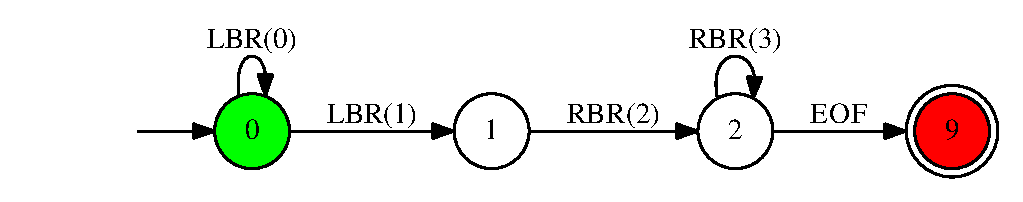
\includegraphics[scale=0.3]{dot/in3.eps}
   }  
   \hfill
    \subfloat[SPPF\label{resultSPPF}]{%
      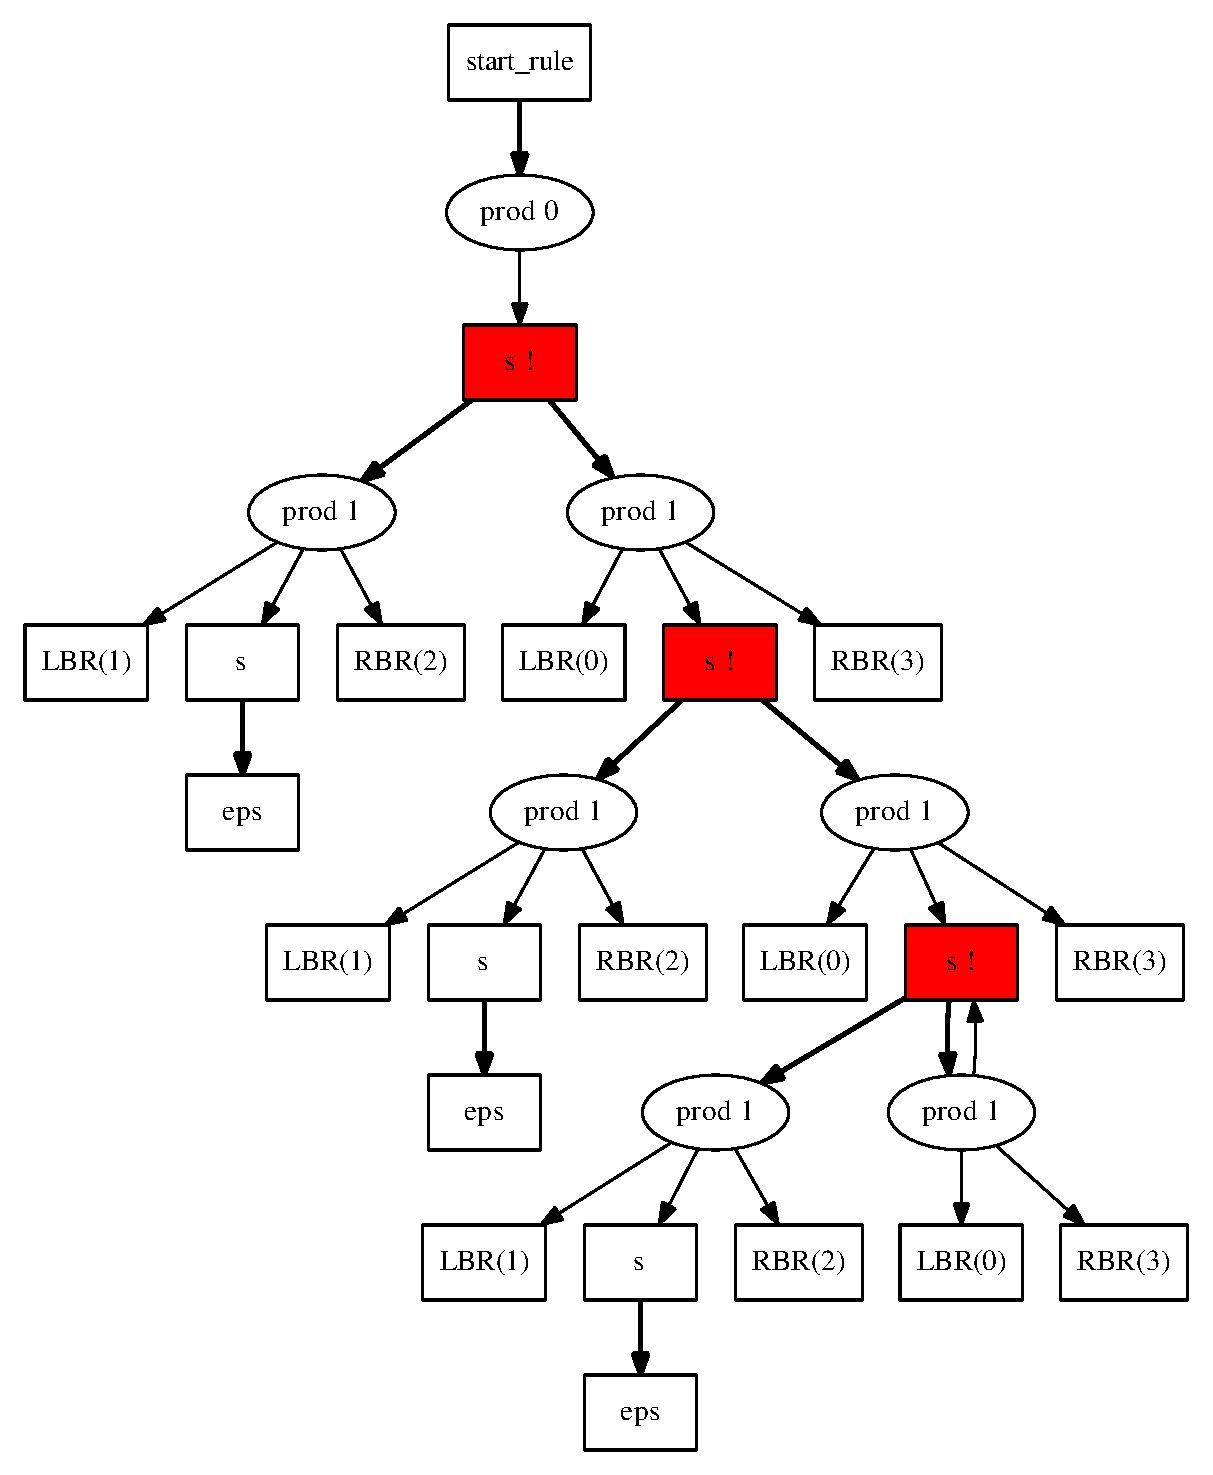
\includegraphics[scale=0.3]{dot/out3.eps}
    }
    \caption{Regular approximation and SPPF}
    \label{fig:SPPFforReg}
 \end{figure}

%\begin{figure}
%    \begin{center}
%        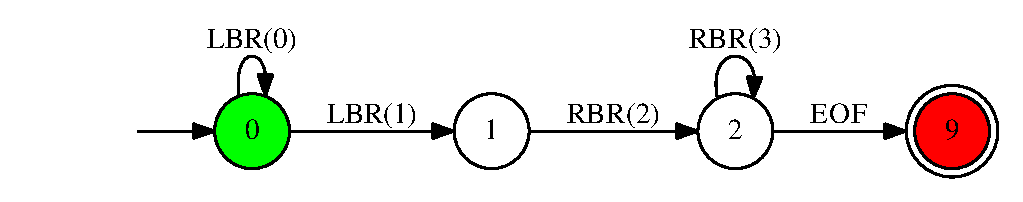
\includegraphics[scale=0.5]{dot/in3.eps}
%    \end{center}
%    \caption{$A_1$ -- input for our algorithm: regular approximation for string-embedded code after tokenization} 
%    \label{faApprox}
%\end{figure}

As it can be seen, some of the words from regular approximation do not belong to the reference language (for example, 
\verb|LBR LBR RBR|). The algorithm ignores such strings and constructs SPPF, which contains derivation trees 
for all recognized strings w.r.t. reference grammar.

%\begin{figure}
%    \begin{center}
%        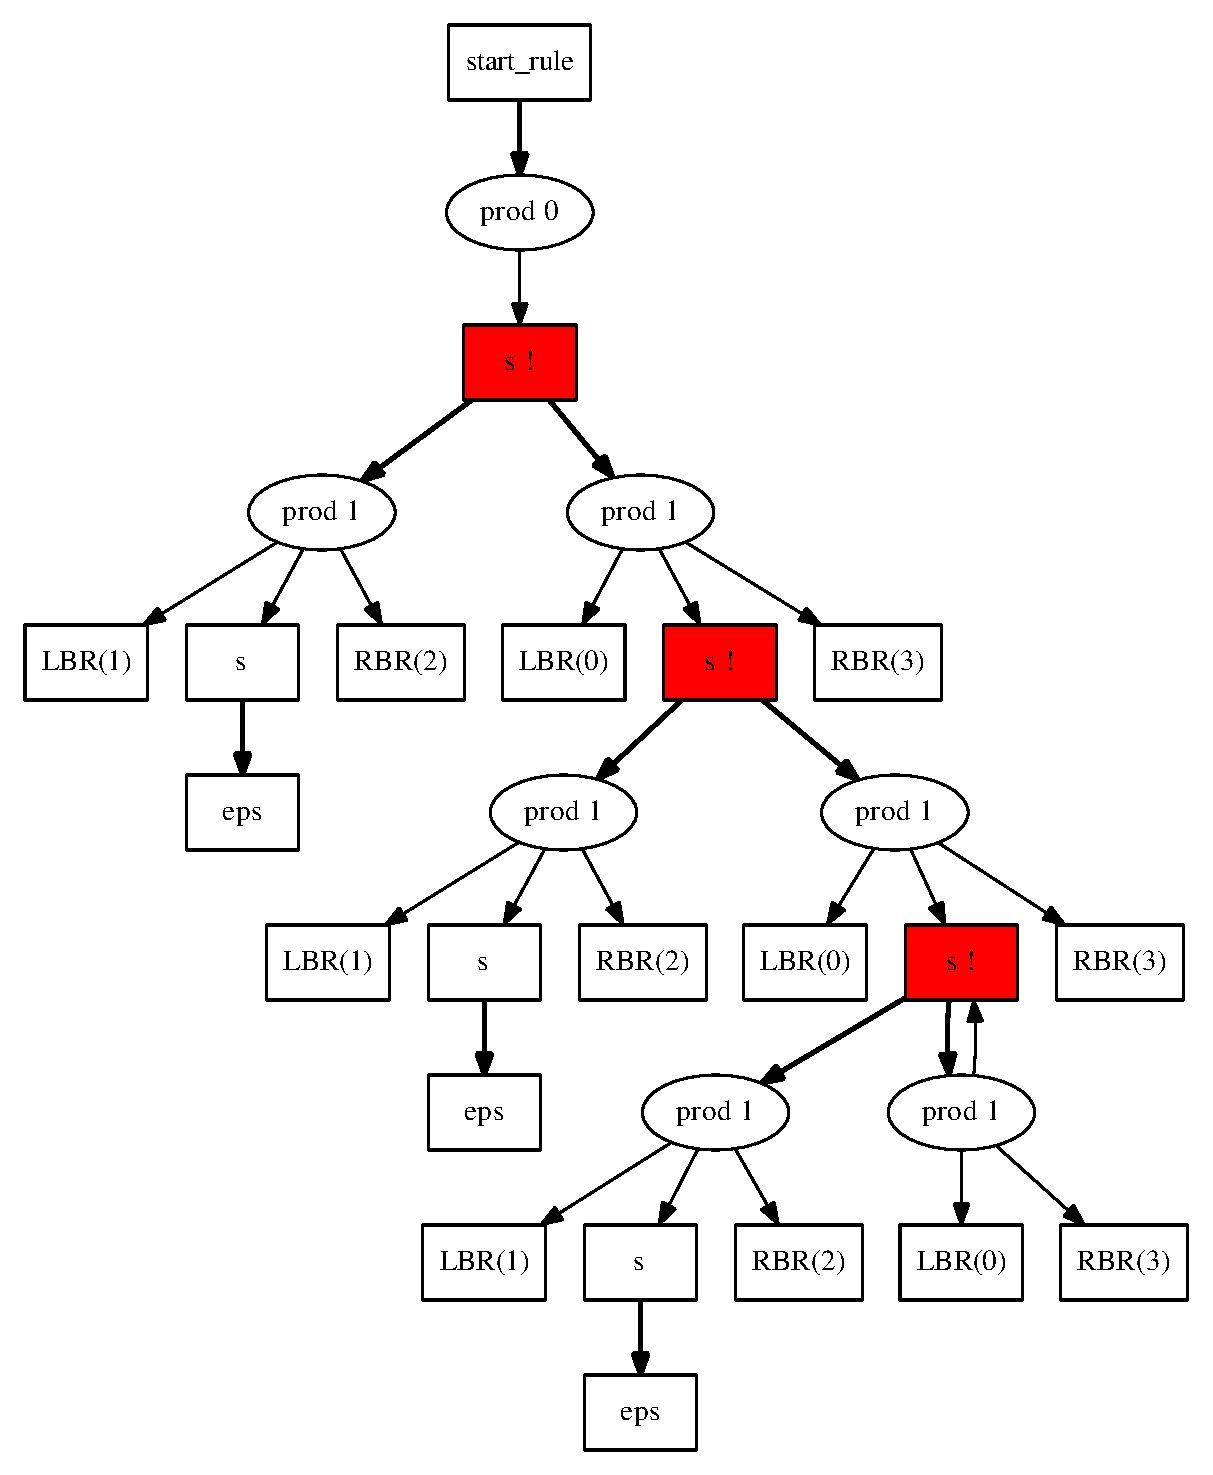
\includegraphics[scale=0.3]{dot/out3.eps}
%    \end{center}
%    \caption{SPPF for input FA presented in figure~\ref{faApprox}}
%    \label{resultSPPF}
%\end{figure}
\pagebreak
\section{\appendixname: RNGLR pseudocode}\label{RNGLRCode}

\begin{algorithm}[]
\begin{algorithmic}[1]
\caption{RNGLR algorithm}
\label{rnglr}
\Function{parse}{$grammar, input$}
  \State{$\mathcal{R} \gets \emptyset$} \Comment{Queue of tuples of GSS vertex, nonterminal, and reduction length}
  \State{$\mathcal{Q} \gets \emptyset$} \Comment{Collection of pairs of GSS vertex and parser state}
  \If{$input = \epsilon$}
    \If{$grammar$ accepts empty input} {report success}
    \Else { report failure}
    \EndIf
  \Else
    \State{\Call{addVertex}{$0, 0, startState$}}
    \ForAll{$i$ in $0..input.Length-1$}
      \State{\Call{reduce}{$i$}}
      \State{\Call{push}{$i$}}
    \EndFor
    \If{$i=input.Length-1$ and there is a vertex in the last level of GSS which state is accepting}
      \State{report success}
    \Else { report failure}
    \EndIf
  \EndIf
\EndFunction
\Function{reduce}{$i$}
  \While{$\mathcal{R}$ is not empty}
    \State{$(v, N, l) \gets \mathcal{R}.Dequeue()$}
    \State{find the set $\mathcal{X}$ of vertices reachable from $v$ along the path of length $(l-1)$}
    \State{or length $0$ if $l=0$}
    \ForAll{$v_{h} = (level_{h}, state_{h})$ in $\mathcal{X}$}
      \State{$state_{t} \gets$ calculate new state by $state_{h}$ and nonterminal $N$}
      \State{\Call{addEdge}{$i, v_{h}, v.level, state_{tail}, (l=0)$}}
    \EndFor
  \EndWhile
\EndFunction
\Function{push}{$i$}
  \State{$\mathcal{Q^{'}} \gets$ copy $\mathcal{Q}$}
  \While{$\mathcal{Q^{'}}$ is not empty}
    \State{$(v, state) \gets \mathcal{Q}.Dequeue()$}
    \State{\Call{addEdge}{$i, v, v.level + 1, state, false$}}
  \EndWhile
\EndFunction
\end{algorithmic}
\end{algorithm}

\begin{algorithm}[]
\begin{algorithmic}[1]
\caption{GSS construction}
\label{RNGLRMain}
\Function{addVertex}{$i, level, state$}
  \If{GSS does not contain vertex $v = (level, state)$}
    \State{add new vertex $v = (level, state)$ to GSS}
    \State{calculate the set of shifts by $v$ and the $input[i+1]$ and add them to $\mathcal{Q}$}
    \State{calculate the set of zero-reductions by $v$ and the $input[i+1]$ and}
    \State{add them to $\mathcal{R}$}
  \EndIf
  \State{\Return{$v$}}
\EndFunction
\Function{addEdge}{$i, v_{h}, level_{t}, state_{t}, isZeroReduction$}
  \State{$v_{t} \gets$ \Call{addVertex}{$i, level_{t}, state_{t}$}}
  \If{GSS does not contain edge from $v_{t}$ to $v_{h}$}
    \State{add new edge from $v_{t}$ to $v_{h}$ to GSS}
    \If{not $isZeroReduction$}
      \State{calculate the set of reductions by $v$ and the $input[i+1]$ and}
      \State{add them to $\mathcal{R}$}
    \EndIf
  \EndIf
\EndFunction
\end{algorithmic}
\end{algorithm}




%\subsection{Part One}


\end{document}
